\documentclass[crop=false]{standalone}
\usepackage{standard}

\begin{document}
  \section{Lösungsmethoden} % (fold)
  \label{sec:loesungsmethoden}



    \subsection{Vorbereitung} % (fold)
    \label{sub:Vorbereitung}

      \subsubsection{Einlesen der Szenendaten} % (fold)
      \label{ssub:einlesen_der_daten}
        \paragraph{STL-Dateiformat}
        Das STL-Dateiformat (engl.: \textit{stereolithography}) beschreibt die Oberfläche von 3D-Körpern mit Hilfe von Dreiecksfacetten.
        Jede Dreiecksfacette wird durch die drei Eckpunkte und die zugehörige Flächennormale des Dreieckes charakterisiert.
        Bei der hier verwendeten Variante handelt es sich um die binäre Form des Dateiformats, da so eine erhebliche Reduktion der Dateigröße erreicht wird.
        Zudem übersteigt die Einlesegeschwindigkeit des binären Formats die des Standardformats um mehrere Größenordnungen.

        Das Einlesen einer STL-Datei wird im C++-Code durch die Klasse \texttt{std::fstream} realisiert.
        Diese Klasse ist in jedem C++-Compiler vorhanden, wie es im Sprachstandard festgelegt ist.
        Zunächst wird durch das Auslesen des Dateikopfes die Anzahl der Dreiecke bestimmt.
        Basierend auf dieser Zahl wird ein Array im Arbeitsspeicher alloziert.
        Mithilfe einer \texttt{for}-Schleife werden dann die Daten jedes einzelnen Dreiecks ausgelesen und im Array gespeichert.
        Im Folgenden ist dieses Verfahren durch ein Codebeispiel gezeigt.

        \inputCodeBlock[title = STL Loader]{code/stl_reader.cc}

        \paragraph{OBJ-Dateiformat}
        OBJ (auch \textit{Wavefront OBJ}) ist ein offenes Dateiformat zum Speichern von dreidimensionalen geometrischen Formen.
        Das Format wird von vielen 3D-Grafikprogrammen unterstützt und ist daher geeignet für die programm- und plattformübergreifende Weitergabe von 3D-Modellen.
        Es handelt sich um ein ASCII-basiertes Dateiformat, welches zeilenweise ausgelesen werden muss.
        Jede Zeile enthält einen Befehl mit den entsprechenden Argumenten.
        Für dieses Projekt wurden nur drei der vielen Befehle verwendet.

        \inputCodeBlock[title = OBJ Kommandos,language=]{code/obj_commands.obj}

        Auch bei diesem Dateiformat wurde die Klasse \texttt{std::fstream} verwendet.
        Für die Eckpunkte, die Normalen und die Flächen wurde jeweils ein eigener Container generiert.
        Bei dem Container handelt es sich um das Template \texttt{std::vector} der C++-Standardbibliothek.
        Durch die Verwendung dieses Templates wird das Hinzufügen eingelesener Daten auch bei Überschreitung des reservierten Speichers effizient durchgeführt.
        Alle Koordinaten wurden mit einfacher Genauigkeit in dem Gleitkommatyp \texttt{float} und alle Referenzen auf Eckpunkte oder Normalen im Ganzzahltyp \texttt{int} gespeichert.
      % subsubsection einlesen_der_daten (end)

      \subsubsection{Ausgabe} % (fold)
      \label{ssub:ausgabe}
        Für die graphische Ausgabe wurde die Bibliothek OpenGL zusammen mit dem Framework GLUT verwendet.
        GLUT erstellt einen OpenGL-Context und dient auch als Window-Manager.
        OpenGL wird benötigt um den Pixelpuffer eines Fensters (Array, indem der Status jedes Pixels eines Fensters gespeichert ist) auf dem Bildschirm auszugeben.

        Um sowohl das Einlesen der Dateiformate als auch die Korrektheit des Raytracers zu testen, wurde die Graphics-Engine von OpenGL genutzt.
        Anhand einiger Standardmodelle, wie dem \textit{Conference Room} in Abbildung \ref{fig:raytracer-example}, konnte die korrekte Funktion der Datei-Loader und der graphischen Ausgabe sichergestellt werden.
        \begin{figure}
          \center
          \begin{subfigure}[b]{0.49\textwidth}
            \center
            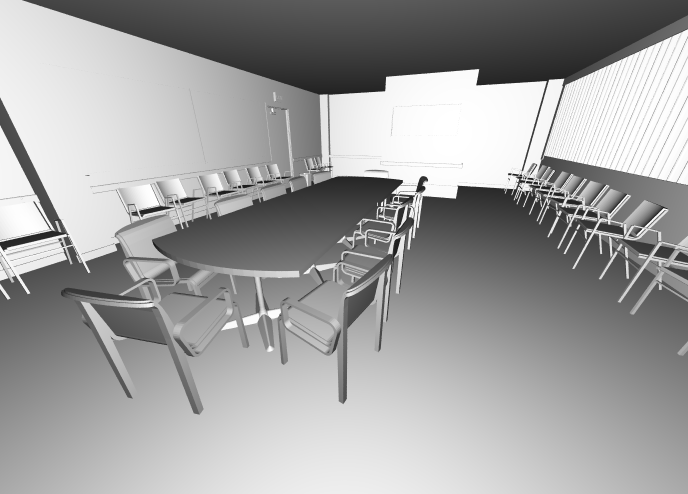
\includegraphics[width=0.95\textwidth]{images/ray_tracer_example.png}
          \end{subfigure}
          \begin{subfigure}[b]{0.49\textwidth}
            \center
            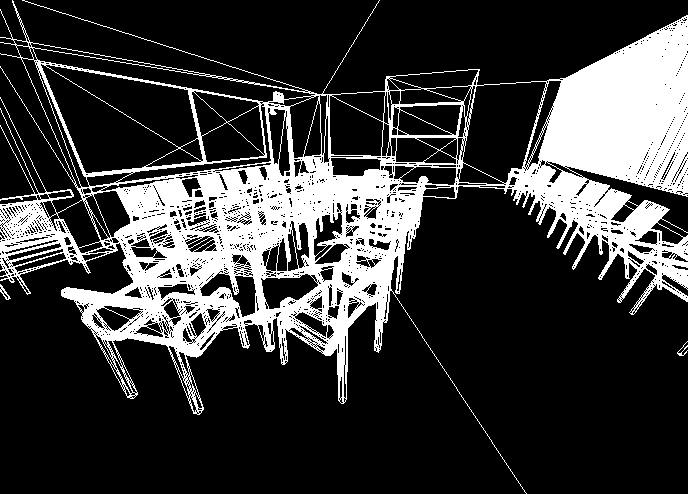
\includegraphics[width=0.95\textwidth]{images/opengl_example.png}
          \end{subfigure}
          \caption{%
            Die Abbildung zeigt die Szene \textit{Conference Room}.
            Auf der linken Seite wurde das Bild mithilfe des Raytracers generiert.
            Die rechte Seite zeigt das \textit{Wireframe} gerendert durch OpenGL.
          }
          \label{fig:raytracer-example}
        \end{figure}
      % subsubsection ausgabe (end)

      \subsubsection{Performance-Analyse} % (fold)
      \label{ssub:performance_analyse}
        Damit die Effizienz der Algorithmen objektiv miteinander verglichen werden konnte, wurde die mittlere Zeitspanne zum Erstellen eines Bildes (Frame) für jeden Algorithmus gemessen.
        Das Reziproke dieser Messgröße wird in der Literatur auch als \textit{frames per second} (FPS) bezeichnet.
        Hierfür wurde innerhalb einer festgelegten Zeitspanne (in der Regel 5 Sekunden) gemessen, wie oft der Pixel Puffer neu berechnet und ausgegeben wurde.
        Der Quotient aus der gesamten Zeitspanne und der Anzahl der erzeugten Frames ist dann die mittlere Zeit, die zur Berechnung des Pixel Puffers benötigt wird.

        Die hohe Komplexität der Szenen resultiert in starken Schwankungen der FPS je nach Position und Richtung der Kamera.
        Die verschiedenen Algorithmen arbeiten in unterschiedlichen Raumbereichen mit unterschiedlicher Effizienz.
        Für eine quantitative Analyse dieser Algorithmen wurden aus diesem Grund vorher festgelegte Kamerapfade verwendet.
        Der Beobachter bewegt sich auf diesen Pfaden und misst für jeden gegebenen Punkt die FPS.
        So können die Stärken und Schwächen der einzelnen Algorithmen ermittelt werden.

        Zum Festlegen der Kamerapfade muss eine Szene zunächst von einem Benutzer analysiert werden, um Bereiche mit hohen FPS-Schwankungen zu finden.
        Hierfür wurde die manuelle Steuerung der Kamera durch den Benutzer ermöglicht.
        Zudem existieren auch hochkomplexe Szenen, die nur durch die manuelle Analyse untersucht werden können.
      % subsubsection performance_analyse (end)
    % subsection vorarbeit (end)

    \subsection{Naiver Algorithmus} % (fold)
    \label{sub:naiver_algorithmus}
      Abbildung \ref{fig:raytracing} stellt eine Skizze des grundsätzlichen Algorithmus dar.
      Für jeden Pixel des Pixelpuffers wird ein Strahl von der Kameraposition durch den Pixel in die Richtung des Bildschirms ausgesendet.
      Jeder dieser Strahlen wird dann mit der Szene auf Schnittpunkte getestet.
      Existiert ein Schnittpunkt, so wird dieser durch weitere Algorithmen dargestellt.
      Existieren mehrere Schnittpunkte, so wird derjenige ausgewählt, der der Kamera am nächsten ist.
      \begin{figure}
        \center
        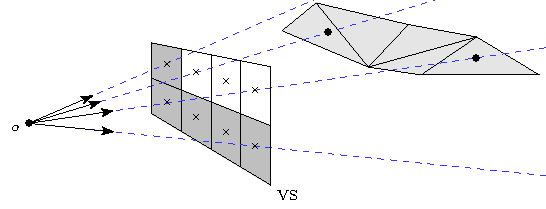
\includegraphics{images/ray_tracing_scheme.pdf}
        \caption{%
          Die Skizze stellt das Raytracing-Verfahren dar.
          Bezüglich eines Beobachtungspunktes $o$ wird durch jeden Pixel eines virtuellen Bildschirms $\mathrm{VS}$ ein Strahl geschossen.
          Die grau melierten Dreiecke stellen dabei die Szene dar.
          Jeder Pixel des virtuellen Bildschirms entspricht einem analogen Pixel des realen Bildschirms.
        }
        \label{fig:raytracing}
      \end{figure}

      Für die Implementierung wurde das Einlesen der Szene als Liste von Dreiecken wie in Abschnitt \ref{ssub:einlesen_der_daten} realisiert.
      Die Kamera konnte mithilfe einer Klasse dargestellt werden.
      In der folgenden Abbildung HIERGROßEFETTEABBILDUNGEINFÜGEN ist die Bedeutung der einzelnen Parameter skizziert.
      Die Position und Ausrichtung der Kamera wurde durch eine positiv orientierte affine Basis im $R^3$ beschrieben.
      Der erste Basisvektor zeigt in die Richtung, die für die Kamera als rechts definiert ist.
      Analoges gilt für den zweiten und dritten Basisvektor bezüglich den Richtungen oben und hinten.
      Der zu einer Kamera gehörige virtuelle Bildschirm wurde durch die Anzahl seiner Pixel $n_\mathrm{w}$ und $n_\mathrm{h}$ in der Breite und Höhe charakterisiert.
      Die Entfernung zur Kamera wurde durch den Öffnungswinkel $\alpha$, unter dem die Höhe des Bildschirms von der Kamera aus zu sehen ist, angegeben.
      Weitere Größen wie die Kantenlänge $p$ eines Pixels im Raum oder das Seitenverhältnis $a$ des virtuellen Bildschirms lassen sich aus den bereits definierten Größen eindeutig berechnen.
      \[
        p = \frac{2\tan \frac{\alpha}{2}}{n_\mathrm{h}}
        \qquad
        a = \frac{n_\mathrm{w}}{n_\mathrm{h}}
      \]

      Die von der Kamera ausgesendeten Primärstrahlen mussten auf Schnittpunkte mit der Szene getestet werden.
      Für jeden Strahl wurden hierfür mithilfe des Möller-Trumbore-Verfahrens die Schnittpunkte mit allen Dreiecken der Szene berechnet.
      Um das genannte Verfahren genauer zu erklären, seien $A,B,C\in R^3$ die Eckpunkte eines Dreiecks, wobei gilt, dass die Menge $\left\{ B-A,C-A \right\}$ linear unabhängig ist.
      Wie sich leicht überprüfen lässt, lassen sich alle Punkte des Dreiecks durch die folgende Parametrisierung beschreiben.
      \begin{align*}
        &M \coloneqq \left\{ (u,v)\in [0,1]^2 \ \middle|\ u+v \leq 1 \right\} \\
        &\varphi\colon M\to \mathds{R}^3 \qquad \varphi(u,v)\coloneqq (1-u-v)A + uB + vC
      \end{align*}
      Die Koordinaten $u$, $v$ und $1-u-v$ werden auch als die baryzentrischen Koordinaten eines Dreiecks bezeichnet.
      Weiterhin nehmen wir an, dass der Strahl durch die folgende Funktion, den Ursprung $o\in\mathds{R}^3$ und die Richtung $d\in\mathds{R}^3\setminus\{0\}$ beschrieben wird.
      \[
        r\colon [0,\infty) \to \mathds{R}^3
        \qquad
        r(t) \coloneqq o + td
      \]
      Für einen Schnittpunkt müssen die baryzentrischen Koordinaten des Dreiecks den gleichen Punkt im Raum wie die Parametrisierung des Strahls beschreiben.
      \[
        o + td = A + (B-A)u + (C-A)v
      \]
      Durch Umbenennung lässt sich diese Gleichung etwas vereinfachen.
      \[
        e_0 = ue_1 + ve_2 - td
      \]
      \[
        e_0 \coloneqq o - A
        \qquad
        e_1 \coloneqq B-A
        \qquad
        e_2 \coloneqq C-A
      \]
      Fasst man nun die Koordinaten $u$, $v$ und $t$ zu einem Vektor zusammen, so lässt sich die Gleichung sehr elegant durch ein Matrix-Vektor-Produkt formulieren.
      \[
        e_0 =
        \begin{pmatrix}
          e_1 &
          e_2 &
          -d
        \end{pmatrix}
        \begin{pmatrix}
          u \\
          v \\
          t
        \end{pmatrix}
      \]
      Dieses lineare Gleichungssystem ist genau dann lösbar, wenn die Determinante der Matrix ungleich Null ist.
      \[
        \begin{pmatrix}
          u \\
          v \\
          t
        \end{pmatrix}
        =
        \begin{pmatrix}
          e_1 &
          e_2 &
          -d
        \end{pmatrix}^{-1}
        e_0
      \]
      Die inverse der Matrix lässt sich analytisch leicht durch Skalar- und Kreuzprodukte beschreiben.
      Diese ermöglichen zudem eine effiziente Berechnung.
      \[
        \begin{pmatrix}
          u \\
          v \\
          t
        \end{pmatrix}
        =
        \frac{1}{\left\langle e_1, d\times e_2  \right\rangle}
        \begin{pmatrix}
          \left\langle d\times e_2 , e_0 \right\rangle \\
          \left\langle e_1\times d , e_0 \right\rangle \\
          \left\langle e_1\times e_2, e_0 \right\rangle
        \end{pmatrix}
        =
        \frac{1}{\left\langle e_1, d\times e_2  \right\rangle}
        \begin{pmatrix}
          \left\langle d\times e_2 , e_0 \right\rangle \\
          \left\langle e_0\times e_1 , d \right\rangle \\
          \left\langle e_0\times e_1, e_2 \right\rangle
        \end{pmatrix}
      \]
      Durch diese Gleichung lassen sich nun die Parameter $u$, $v$ und $t$ bestimmen.
      Es muss überprüft werden, ob diese auch die Bedingungen der Parametrisierungen erfüllen.
      \[
        \left\langle e_1, d\times e_2  \right\rangle \neq 0
        \qquad
        u,v,t \geq 0
        \qquad
        u+v\leq 1
      \]
      Sind die Bedingungen erfüllt, so liegt ein Schnittpunkt vor.
      Implementiert wurde dieser Algorithmus durch den folgenden Quelltext.

      \inputCodeBlock[title=test]{code/moeller_trumbore_intersection.cc}

    % subsection naiver_algorithmus (end)
  % section lösungsmethoden (end)
\end{document}